%\documentclass[PhD]{iitddiss}
%\documentclass[MS]{iitddiss}
% \documentclass[MTech]{iitddiss}
\documentclass[Dual]{iitddiss}
%\documentclass[BTech]{iitddiss}
% \documentclass[Other]{iitddiss}
% IF YOU USE THE OTHER OPTION, THEN YOU MUST FILL OUT THE PROGRAM OPTION BELOW TOO
\program{My Fancy Degree}

% \usepackage{times}
 \usepackage{t1enc}

\usepackage{graphicx}
\usepackage{hyperref} % hyperlinks for references.
\usepackage{amsmath} % easier math formulae, align, subequations \ldots
\usepackage[english]{babel}
\usepackage[utf8]{inputenc}
\usepackage{natbib}
\usepackage{fancyhdr}
 \linespread{1.2}

\pagestyle{fancy}
\renewcommand{\sectionmark}[1]{\markright{\thesection\ #1}}

\fancyhf{}

\rhead{\fancyplain{}{\thepage}} % predefined ()
\lhead{\fancyplain{}{\rightmark}} % 1. sectionname, 1.1 subsection name etc
\cfoot{\textcopyright \text{ } \the\year, \emph{Indian Institute of Technology Delhi}}
\renewcommand{\footrulewidth}{0.4pt}
\begin{document}


%%%%%%%%%%%%%%%%%%%%%%%%%%%%%%%%%%%%%%%%%%%%%%%%%%%%%%%%%%%%%%%%%%%%%%
% Title page

\title{Knowledge Base Adaptation for Task Oriented Dialog}

\author{Nikhil Gupta}
\advisor{Prof. Mausam}
\entrynumber{2014CS50462}
\date{June 2019}
\department{Computer Science and Engineering}

%\nocite{*}
\maketitle

%%%%%%%%%%%%%%%%%%%%%%%%%%%%%%%%%%%%%%%%%%%%%%%%%%%%%%%%%%%%%%%%%%%%%%
% Certificate
\certificate

\vspace*{0.5in}

\noindent This is to certify that the thesis titled {\bf Knowledge Base Adaptation for Task Oriented Dialog}, submitted by {\bf Author},
  to the Indian Institute of Technology, Delhi, for
the award of the degree of {\bf Master of Technology}, is a bona fide
record of the research work done by him under our supervision.  The
contents of this thesis, in full or in parts, have not been submitted
to any other Institute or University for the award of any degree or
diploma.

\vspace*{1.5in}

\begin{singlespacing}
\hspace*{-0.25in}
\parbox{2.5in}{
\noindent {\bf Mausam} \\
\noindent Professor \\
\noindent Dept. of Computer Science\\
\noindent IIT-Delhi, 600 036 \\
}
\hspace*{1.0in}
\end{singlespacing}
\vspace*{0.25in}
\noindent Place: New Delhi\\
Date: 28th June 2019


%%%%%%%%%%%%%%%%%%%%%%%%%%%%%%%%%%%%%%%%%%%%%%%%%%%%%%%%%%%%%%%%%%%%%%
% Acknowledgements
\acknowledgements
I would like to extend thanks to Microsoft for graciously providing me a VM to work on.
I would thank my advisor Mausam for his constant support and insights on this project. 
I would like to thank Dinesh for his suport and effort and guiding me along the way for this journey.

Thanks to all those who made \TeX\ and \LaTeX\ what it is today.
\pagebreak

%%%%%%%%%%%%%%%%%%%%%%%%%%%%%%%%%%%%%%%%%%%%%%%%%%%%%%%%%%%%%%%%%%%%%%
% Abstract

\abstract
Dialog systems or chatbots are computer programs that can interact with humans either using a speech interface or text interface. 
% Building dialog systems are gaining popularity due to two major reasons. One to accomplish a task, such as purchasing a mobile phone from Amazon, internet users prefer a simple chat interface compared to navigating through websites or a mobile app. Two, mobile phone users spend most of their time using email or messaging applications.
Based on the application, dialogs systems can be divided into two categories: open domain and task oriented. Dialog systems that converse with an intention to accomplish a task such as recommending a restaurant or booking a flight tickets are task oriented dialog systems. Such systems gennerally need to consult a Knowledge Base (KB) with stored information to accomplish the task. End-to-end neural networks trained for these task-oriented dialogs are expected to be immune to any changes in this KB which can evolve with time. However, existing approaches breakdown when asked to handle such changes. The failure is mostly due to the inability to handle Out-of-Vocabulary (OOV) words and the inability to perform simple reasoning over the knowledge base results such as suggest without repetition and sorting based on a field.
% and a simple analysis shows that there exists a huge gap when evaluated using task specific metrics.
% Research in open domain dialog systems have progressed to a state where given a large corpus of conversation logs, the deep learning models can learn to converse end-to-end without the need of defining hand crafted, domain specific rules. Most of the research on modeling dialog systems has been focused on only learning to converse by remembering how conversation are sustained in the training examples. There has been very little work around on how to learn an end-to-end task oriented dialog system that requires access to a knowledge base to accomplish a given task. 

% The existing end-to-end task oriented dialog system which uses knowledge base perform well only on open domain dialog system evaluation metrics, a simple analysis shows that there exists a huge gap when evaluated using task specific metrics. The failure is mostly due to the inability to handle OOV words, inability to perform simple reasoning over knowledge base results such as suggest without repetition and sorting based on a field over.



% We first solve the limitations in the existing model by proposing a deep network that can consume knowledge base results and perform basic reasoning. To accomplish this we propose a hierarchical attention network with the ability to perform location based addressing. The overall goal of this research is to learn a usable task oriented dialog system from long human-human chat transcripts. To achieve the goal, we propose to solve the following problems: one, dialog system that can perform complex reasoning such as inferring from more than one knowledge base result to generate a response. The existing systems access the knowledge base just once during the conversation, we propose to extend this by modeling a system that is capable to conversing by accessing the knowledge base more than once. For example, when purchasing a product such as mobile phone, the user describes her requirements,  based on the mobile phones available in the knowledge base, the system should help narrow down the option based on the results. We then wish to work on knowledge bases that contains semi-structured fields along with the structured fields. Finally, we wish to learn a usable dialog system using human to human conversations.

% \noindent The Knowledge Base (KB) used for real-world applications, such as booking a movie or restaurant reservation, keeps changing over time. End-to-end neural networks trained for these task-oriented dialogs are expected to be immune to any changes in the KB. However, existing approaches breakdown when asked to handle such changes. 
We studied the correlation between the learned language model and the knowledge base incorporation and conjectured that we must strive to create a system that learns both mutually exculsive of the other, i.e. in a disentangled manner.
We propose an encoder-decoder architecture (\sys) with a novel Bag-of-Sequences (\textsc{BoSs}) memory, which facilitates such disentangled learning. Consequently, the KB can be modified with new knowledge without a drop in interpretability. We find that \sys\ outperforms state-of-the-art models, with considerable improvements (\textgreater10\%) on bAbI OOV test sets and other humsan-human datasets. We also systematically create adversarial attacks that introduce modifications to the KB in an attempt to measure the extent of disentanglement and show that \sys\ remains robust to all such attacks.
% We also systematically modify existing datasets to measure disentanglement and show \sys\ to be robust to KB modifications.

Generally the training set dialogs in task-oriented systems use an explicit API for KB retreival which must be manually annotated within the dialogs themselves. We attempt to go one step further by reducing the amount of annotations needed to train such task-oriented dialogs by predicting the correct API without it being explicitly mentioned. We generate this API using an RL-based decoder. The results from this API are then used to generate responses by our response decoder which serve as feedback (reward) to train the RL decoder. We created a novel architecture that would be capable to mitigte two critical problems: data bias (multiple APIs fetch similar KB results) and length bias (preference of the RL decoder to predict short length APIs over longer ones, despite worse results). Our system was successfully able to achieve similar performance on the unannotated dataset as compared to the fully API annotated dataset.
% which trains based on the feedback (reward) it receives on its ability to generate correct responses on the results extracted by the predicted API call.

\pagebreak

%%%%%%%%%%%%%%%%%%%%%%%%%%%%%%%%%%%%%%%%%%%%%%%%%%%%%%%%%%%%%%%%%
% Table of contents etc.

\begin{singlespace}
\tableofcontents
\thispagestyle{empty}

\listoftables
\addcontentsline{toc}{chapter}{LIST OF TABLES}
\listoffigures
\addcontentsline{toc}{chapter}{LIST OF FIGURES}
\end{singlespace}
\pagebreak

% The main text will follow from this point so set the page numbering
% to arabic from here on.
\pagenumbering{arabic}

%%%%%%%%%%%%%%%%%%%%%%%%%%%%%%%%%%%%%%%%%%%%%%%%%%%%%%%%%%%%%%%%%%%%%%
% Introduction
\chapter{INTRODUCTION}
%%%%%%%%%%%%%%%%%%%%%%%%%%%%%%%%%%%%%%%%%%%%%%%%%%%%%%%%%%%%%%%%%%%%%%
% Overview
\section{Overview}
Dialog systems, also referred to as chatbots or virtual agents are systems that can converse with a human to help with their informational needs. Dialog systems are used in a wide range of applications such as personal assistants in mobile phones, technical support services, chit chat, product enquiries, IVR systems and entertainment. Some of the popular dialog systems include Apple's Siri, Google Now, Microsoft's Cortana, Amazon's Alexa and Google's Smart Reply. Most of the dialog systems that are being used for real word applications are hand crafted by a dialog designers and also very specific to a domain. Even though using such hand crafted rules provides the flexibility to build a interpretable dialog system, it require a great amount of effort for the dialog designer to create one from scratch for a new domain. This extra effort also transcends to scenarios where the existing chatbot's capability has to be extended or improved.

% Recent advancements in the field of neural networks has shown us that data-driven approaches outperform systems with custom hand crafted features. This has been proven for a number of NLP tasks such as part of speech tagging, named entity recognition, speech recognition, etc. This trend is now being observed in the area of building dialog systems. Research on data driven approaches for modeling dialogs have started to shadow the research around improving the traditional hand crafted dialog systems. The data driven approaches have the ability to learn to mimic a human with just access to a large corpus of conversation logs. The system learnt using data driven approaches can at best be used to provide suggestions to possible next responses or provide context based auto complete features in social media, email client or chat applications. For example, the \textit{smart reply} option in GMail. This option scans the email conversation so far and suggests three possible responses to reply with. These systems are far from performing a full fledged conversation and help accomplish user's goal.

Dialog systems can be largely differentiated into two categories, namely, open domain and task-oriented.

\noindent {\bf Open Domain}: Dialog that doesn't involve any underlying task. As a result it is not domain specific and is often broad and unstructured. For example, normal chit-chat and language learning.

\noindent {\bf Task-Oriented}: Dialog where an agent converses with a user with the goal of accomplishing a specific task and often interact with a knowledge-base (KB). For example, a restaurant reservation agent \cite{hen2014word} will be grounded to a KB that contains the names of restaurants, and their details.  

The focus of this thesis will be to improve the ability of task-oriented dialog systems to generalise over its KB.
In real-world applications, the KB information could change over time. For example, (1) a KB associated with a movie ticket booking system gets updated every week based on new film releases, and (2) a restaurant reservation agent, trained with the knowledge of eateries in one city, may be deployed in other cities with an entirely different range of establishments. In such situations, the system should have the ability to conform to new-found knowledge unseen during its training. Ideally, the training algorithm must learn to disentangle the language model from the knowledge interface model. This separation will enable the system to generalize to KB modifications, without a loss in performance.  

Moreover, for achieving good progress towards the user's task, the agent must also retain the ability to draw inferences based on past utterances and the KB. Notably, we find that existing approaches either achieve this disentanglement or effective progress towards the task, but not both.  

For instance, Mem2Seq \cite{mem2seq} exhibits satisfactory performance when tested on the training KB. It represents the dialog history and the KB knowledge as a \emph{bag of words} in a flat memory arrangement. This enables Mem2Seq to revisit each word several times, as needed, obtaining good performance. But at the same time, flat memory prevents it from capturing any surrounding context -- this deteriorates its performance rapidly when the amount of new unseen information in the KB increases, as shown in Figure \ref{fig:camrest}. On the other hand, the performance of copy augmented sequence-to-sequence network (Seq2Seq+Copy) \cite{eric2017copy}, is robust to changes in the KB, but fails to achieve acceptable task-oriented performance. It captures context by representing the entire dialog history as one continuous \emph{sequence}.
However, it can be difficult for a sequence encoder to reason over long dialogs found in real-world datasets and its ability to learn the task gets hampered.  

%%%%%%%%%%%%%%%%%%%%%%%%%%%%%%%%%%%%%%%%%%%%%%%%%%%%%%%%%%%%%%%%%%%%%%
% Problem Definition
\section{Problem Definition}
We now define the scope of the problem we wish explore, by answering the following questions: 1) \textit{what is end-to-end learning ?}, 2) \textit{What is are task oriented dialog systems?} and 3)\textit{why is knowledge base necessary ?}

\textbf{End-to-End Learning}:  While building a dialog system, the components could either be built using hand crafted rules or can also be statistical machine learning model that learns from a provided set of examples (data-driven). A complete dialog system can thus have some components that are built using rules and some that are learnt using data driven approaches. As mentioned previously, not all dialog system built needs to have all three components, in some cases, the designer can decide to combine both dialog manager and the NLG into a single modules. This way the component can be learnt by using a set of (NLU output, expected natural language response) pairs. Even though this bypasses the need for explicitly annotating the dialog manager output for each dialog exchange, the complexity of the module increases thereby demanding a lot more data to train. The approach where all the three components are combined together and examples of (user input in natural language, expected response in natural language) pairs are used to learn a dialog model, is referred to as \textit{end to end} dialog models. Note that in end to end learning, the intermediate output space may be  defined, but examples are not annotated with expected intermediate outputs.

\textbf{Task Oriented}: Application of dialog systems can be broadly categorized into two types: open domain (non-task oriented) dialog systems and task oriented dialog systems. The main difference between the two approaches is that, the objective of the former is usually broad and not well defined (abstract), where as the objective of the latter is  narrow and well-defined. For example, the restaurant reservation domain dialogs falls under task oriented systems. The goal could be, given a set of options (price range: moderate, location: east Delhi), the system should be able to suggest the right restaurant that is acceptable by the user. A large portion of the research in data driven approaches for dialog modeling has been around non-task oriented. Some examples include chit-chat and language learning. Applications such as restaurant reservation, flight booking, travel enquiry and bus enquiry belong to the task-oriented setting.  One advantage of working on task oriented dialogs over the non-task oriented is easy of defining an evaluation techniques to measure the performance of the system. The performance of the system can be measure by the percentage of conversations where the dialog system was able to help the user achieve her goal. 

Question answering systems and task oriented dialog systems are very similar to each other. The major difference between the two is that, in question answering all details necessary to achieve the task are provided in a single shot, where as in task oriented dialog, the user does not necessarily provide all the information required to achieve the task and its the job of the dialog system to collect them. The dialog systems also provides the ability to carry over context when switching between tasks.

\textbf{Knowledge Base in the Loop}: These are the subset of dialog system that requires access to a knowledge base to respond to user input. Some examples are  using a database of bus running status by a bus enquiry system, using a knowledge base of restaurants by a restaurant reservation systems and using a open domain knowledge base such as Freebase for a dialog system that answers general knowledge questions. There has been a large amount of work on using databases in systems that use hand crafted features for modeling dialog. The community has recently (in 2017) started to explore the area of learning data-driven dialog models grounded by a knowledge base.

To summarize, the goal of our research is to build a dialog system that takes as input 1) a large set of task oriented conversation logs between a user and an agent/domain expert, 2) a knowledge base used to generate agent response and learn a dialog system that can mimic the agent to accomplish a user's task.  

We propose \sys, a novel network that effectively disentangles the language and knowledge models, and also achieves state-of-the-art performance on three existing datasets.  

To achieve this, \sys\ makes two design choices. First, it encodes the conversational input as a {\em bag of sequences} (\textsc{BoSs}) memory, in which the input representation is built at two levels of abstraction. The \emph{higher level} flat memory encodes the KB tuples and utterances to facilitate effective inferencing over them. The \emph{lower level} encoding of each individual utterance and tuple is constructed via a sequence encoder (Bi-GRU). This enables the model to maintain the sequential context surrounding each token, aiding in better interpretation of unseen tokens at test time. Second, we augment the standard cross-entropy loss used in dialog systems with an additional loss term to encourage the model to only copy KB tokens in a response, instead of generating them via the language model. This combination of sequence encoding and additional loss (along with dropout) helps in effective disentangling between language and knowledge.  

We perform evaluations over three datasets -- bAbI \cite{BordesW16}, CamRest \cite{wenEMNLP2016}, and Stanford Multi-Domain Dataset \cite{Ericsigdial}. Of these, the last two are real-world datasets. We find that \sys\ is competitive or significantly better on standard metrics in all datasets as compared to state-of-the-art baselines. We also introduce a {\em knowledge adaptability} (KA) evaluation, in which we systematically increase the percentage of previously unseen entities in the KB. We find that \sys\ is highly robust across all percentage levels. Finally, we also report a human-based evaluation and find that \sys\ responses are frequently rated higher than other baselines.

%%%%%%%%%%%%%%%%%%%%%%%%%%%%%%%%%%%%%%%%%%%%%%%%%%%%%%%%%%%%%%%%%%%%%%
% Motivation
\section{Motivation}
In this section, we motivate our problem by clearly define the gap between what the state-of-the-art, data driven approaches for dialog learning is capable of and what it takes to build a usable end-to-end task oriented dialog system that requires knowledge base in the loop.\\

\noindent
\textbf{Why cant already proven non-task oriented models be used}

While end to end non-task oriented (open domain) dialog systems are being used in real world applications \cite{smartreply}, designers still prefer using hand crafted rules for modeling task oriented dialogs. The main reason for success in non-task oriented setting is that, models have largely been evaluated (and applied) in scenarios where, given the conversation so far the system is expected to predict just the immediate next response. Such modeling requires the system to learn a language model and a mapping from the context to the response. But in case of task oriented settings, the requirements/expectations are much more. It is not just required to generate the next utterance based on the context, but understand the global picture of what the task is, what all details are necessary to finish the task, what is the optimal way or strategy to request for missing details and then decide what the next utterance should be. Also, in chit chat bot (non-task oriented) making a mistake in a single turn is not very costly, where as in flight booking system (task-oriented) making a single mistake (mis-interpreting a source city) could turn out to be very costly. Even though a large section of real world applications such flight booking, tourist enquiry system, technical service support, basic medical consultations fall under this category, there has been very little focus so far.

In addition to task oriented setting, when a knowledge base is added into the loop, the system should now also be able to learn when to query a knowledge base, how to incorporate the results from the knowledge base into the conversation. This makes the problem much harder. Hence models that have been proven to work on non-task oriented systems cannot be used for task-oriented applications.\\

\noindent
\textbf{Limitations of state-of-the-art task oriented approaches}

There has been very little progress made end-to-end task oriented dialogs, as most of the proposed approaches has been around using hand crafted rules to either build the entire system, or to define the structured space of each sub-components output. The only work published so far on end to end task oriented conversation has the following limitations:
\begin{enumerate}
\item Both the human and the agent utterances in the dataset are fabricated using rules. This simulated dataset is very simple compared to human to human conversation logs.
\item The system performance is has acceptable accuracy on  non-task oriented evaluation metrics, but the performance is very poor on task oriented evaluation metrics
\item The system is unable to learn simple patterns (that are exhibited in the train corpora) required to perform a task oriented dialog. Some simple patterns are listed below:
\begin{itemize}
\item construct responses based on results from the database. In fact some responses have results that are not in the set of results retrieved from the database
\item not repeating already suggested options
\item retrieve simple relations from set of database results (such as phone number of a restaurant, address of a restaurant)
\end{itemize}  
\item the approach assumes the database does not change over time and all possible field values are known in advance, it has no support for field values that have never been encountered so far (OOVs)
\item The system proposed has a very limited view of the knowledge base. It assumes that it can only perform simple {\emph SELECT} operation with {\emph WHERE} clauses over the knowledge base
\end{enumerate} 

%%%%%%%%%%%%%%%%%%%%%%%%%%%%%%%%%%%%%%%%%%%%%%%%%%%%%%%%%%%%%%%%%%%%%%
% Contributions
\section{Contributions}

Overall, our contributions are:

\begin{enumerate}
    \item We propose \sys, a novel architecture to disentangle the language model from knowledge incorporation in task-oriented dialogs.
    \item We introduce a {\em knowledge adaptability} evaluation to measure the ability of dialog systems to scale performance to unseen KB entities.
    \item Our experiments show that \sys\ is competitive or significantly better, measured via standard metrics, than the existing baselines on three datasets.
\end{enumerate}

We release our code and {\em knowledge adaptability} (KA) test sets for further use by the research community. \url{ https://github.com/dair-iitd/BossNet}.


\pagebreak

%%%%%%%%%%%%%%%%%%%%%%%%%%%%%%%%%%%%%%%%%%%%%%%%%%%%%%%%%%%%%%%%%%%%%%
% Background
\chapter{BACKGROUND}
\section{Related Work}

Dialog systems can be broadly divided into two categories: open domain \cite{vinyals2015neural,serban2016building} and task-oriented dialog systems. Open domain systems generate responses based on just the dialog history, whereas the task-oriented systems generate responses based on the dialog history and a KB associated with the task. 

Task oriented dialogs systems can be further divided into two: modular and end-to-end trainable dialog systems. Modular dialog systems \cite{wen2017network,williams2017hybrid,williams2007partially} require intermediate supervision on dialog transcripts to train each of its modules. Our work falls under end-to-end trainable dialog systems, which requires just the dialog transcripts and no intermediate supervision to train. We discuss end-to-end trainable neural models along two dimensions: 1) decoding: how the response is retrieved or generated and 2) encoding: how the dialog context (dialog history and KB tuples) are represented. 

Most of the existing approaches \cite{BordesW16,liu2017gated,seo2016query,wu2017end} {\em retrieve} a response from a pre-defined set. These methods are generally successful when they have to provide boilerplate responses -- they cannot construct new responses or use words not seen during training. 
To improve upon these, generative approaches are used where the next response is {\em generated} one word at a time \cite{eric2017copy,mem2seq}. These approaches also benefit the OOV problem by incorporating the ability to copy words from the input \cite{vinyals2015pointer,gu2016incorporating}. This copy mechanism has also found success in summarization \cite{nallapati2016abstractive,see2017get} and machine translation \cite{ptr-unk}. \sys\ is a copy incorporated generative approach.

%The dialog context consists of utterances in the past and KB tuples. 
% For encoding, existing approaches either represent the dialog context as {\em set of sets} \cite{mem2seq,BordesW16,liu2017gated} or {\em sequence of sequences} \cite{eric2017copy,ptr-unk}. {\em Set of sets} represents past utterances as a bag of words making it difficult to capture context and work with words not seen during training. {\em Seq of seqs} enforces an order over the set of KB tuples making it harder to perform inferencing over multiple KB tuples. \sys\ uses a {\em set of seqs} representation, which can both capture word contexts and perform inferencing over KB tuples.

For encoding, some approaches represent the dialog history as a sequence \cite{eric2017copy,ptr-unk}. Unfortunately, using a single long sequence for encoding also enforces an order over the set of KB tuples making it harder to perform inferencing over them. Other approaches represent the dialog context as a bag. Original Memory Networks \cite{BordesW16} and its extensions encode each memory element (utterance) as an average of all constituent words -- this cannot point to individual words, and hence cannot be used with a copy mechanism. Mem2Seq encodes each word individually in a flat memory. Unfortunately, this loses the contextual information around a word, which is needed to decipher an unseen word. In contrast, \sys\ uses a bag of sequences encoding, where KB tuples are a set for easier inference, and also each utterance is a sequence for effectively learning when to copy. We go into further detail below highlighting the differences between the two models.


%Attention over hierarchical representation of sentences and words has been used in document classification \cite{yang2016hierarchical} and abstractive text summarization \cite{nallapati2016abstractive}. These representations defines the document as a sequence of sentences while we propose a set to better represent KB tuples.

\subsection{Comparison with Mem2Seq}
\label{sec:relatedmem2seq}
The closest to our model is the recently introduced Mem2Seq \cite{mem2seq}, which also combines the multi-hop reasoning of memory networks with the generative decoding augmented with a copy mechanism. While similar in spirit to \sys, there are significant differences in the two architectures. We illustrate these with Figure \ref{fig:intro}, which shows an example dialog along with an associated KB in both Mem2Seq and \sys\ memories. %Figure \ref{fig:intro}b shows how the dialog is represented in the Mem2Seq memory.

First, the memory in Mem2Seq is a flat representation which operates in part at utterance level and in part at word level. In particular, the individual words of a user/machine utterance are stored in their own memory cells, whereas a KB tuple gets only one memory cell -- the aggregation is done in a bag of words fashion, using words in the entire tuple. For example, the memory element \textit{m1} contains a full KB tuple and \textit{m15} contains only the word ``french'' from the second user utterance.

This implies that Mem2Seq's copy mechanism can only point to a specific KB tuple, but cannot point to a specific constituent of the tuple. This forces Mem2Seq to make a second modeling choice, of allowing only the ``object'' entity of a tuple to be used in the next response. These choices result in three limitations of Mem2Seq, regarding the scenarios in which Mem2Seq can be useful. 


\begin{figure}[t]
\centering
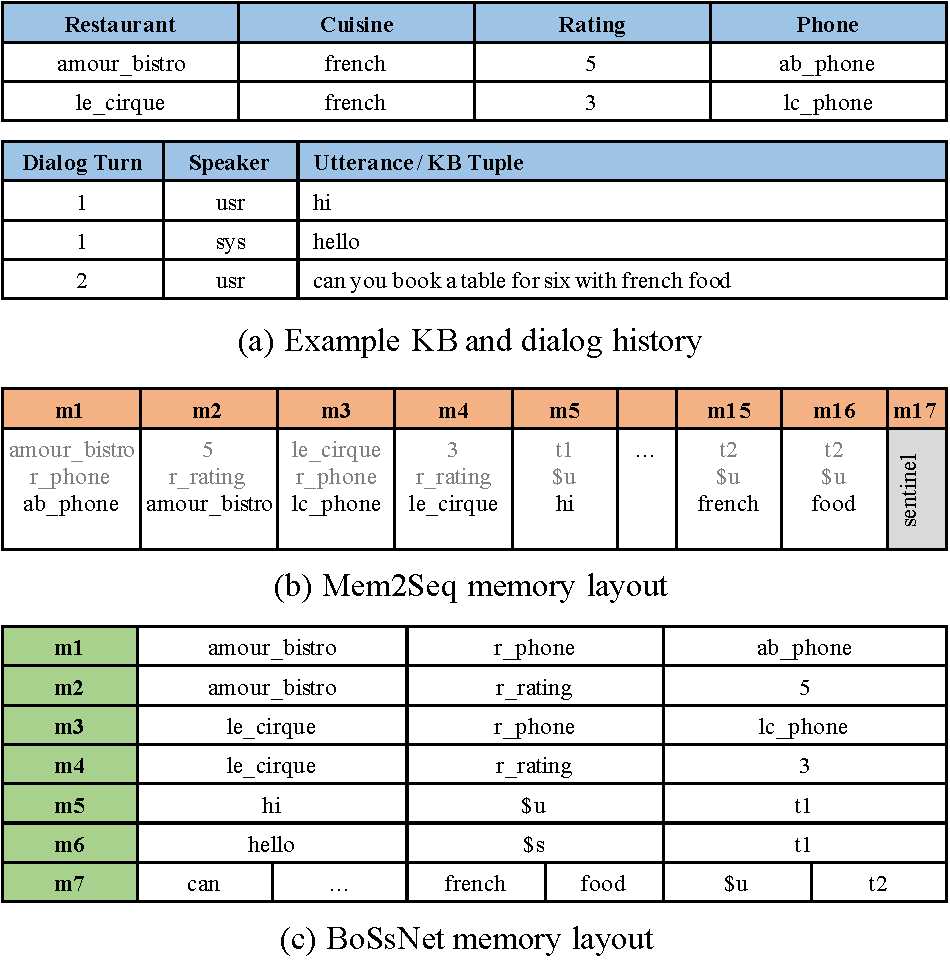
\includegraphics[scale=0.8]{assets/figures/mem2seq.pdf}
\caption{(a) an example dialog with history and KB tuples. (b) an illustration of Mem2Seq memory. (c) an illustration of \sys\ memory}
\label{fig:intro}
\end{figure}

%Our model has the following differences when compared to Mem2Seq: 1) The memory in Mem2Seq has a flat representation whereas we propose a hierarchical representation. 2) The performance of Mem2Seq is dependent on the ordering of KB tuples (subject or object), while the performance of \sys\ is independent of any such ordering. 

% Describe the memory layout
% Each memory element contains either a KB tuple or a word from an utterance in the dialog history. For example, 

% Describe problem #1 and #2
First, Mem2Seq expects each tuple to be serialized by the KB API in way that the object always comes last. This may or may not always be in control of the neural model. Second, because each utterance word has a unique memory cell. it loses the context in which the word was mentioned. As a result, the model cannot learn that ``french'' and other cuisines are usually followed by the word ``food''. This causes poor generalization where the model has to understand an OOV word from the user utterance (e.g., a new cuisine or city name). 
% The vector representation of each memory element is computed using a bag-of-words model. Thus the memory structure prevents the model to generalize by learning clues from the context. 

% Describe problem #3
Finally, the model design dictates that the subject or the predicate from a KB fact can never be copied during the decode step. This adds severe limitations in practical settings. For example, the KB results in the original bAbI dataset \cite{BordesW16} came in format of {\em attribute(restaurant\_name, restaurant\_attribute)}. Since restaurant name is never an object, Mem2Seq would never be able to copy it when making recommendations. As a result, experiments with Mem2Seq necessitated a training data preprocessing, in which all rating facts had to be inverted into {\em rating(restaurant\_rating, restaurant\_name)}, so that the name could become an object and could be copied. 

We believe that this adds severe limitations on the scenarios in which Mem2Seq is applicable. We perform several experiments on the original (unprocessed) datasets to highlight the loss in performance due to these modeling choices. 
In contrast, \sys\ uses a hierarchical memory that can copy {\em any} word from the whole dialog history (see Figure \ref{fig:intro}(c)). It models each cell as a {\em sequence} of words, which also enables it to learn contextual cues for each word, leading to better OOV generalization. 

%The designer needs to carefully choose how a tuple should be placed in the memory. In the example, the object of \textit{r\_phone} (placed at the bottom) is chosen to be the word to copy, while the subject is chosen for \textit{r\_rating}. The placement is dictated by what needs to be copied while generating the response. In the experiments, how ordering affects its performance.

%In the dialog bAbI dataset \cite{BordesW16}, the name of the restaurant and the phone numbers are needed to be copied. Mem2Seq will not be able to generate a response such as ``amour_bistro has a rating of 5'' as the rating object is not addressable by the copy mechanism. 

%Also, if a word occurs more than once in the memory, only the last occurrence of the word is used for computing the copy distribution. This makes the system depend on the order in which KB tuples are placed in the memory
%\todo{Does it fit better now ?}

\section{Components Survey}

\sys\ architecture has a {\em multi-hop encoder}, and a {\em pointer network} decoder with a {\em hierarchical attention} over the memory. The extended architecture has an {\em RL-based API decoder} with mixed on-policy and off-policy sampling. We briefly survey these strands of related research.

\vspace{0.5ex}
\noindent
\textbf{Multi-hop Networks} reason over a sequence of sentences fed as input. A hop refers to reading the sentences and generating a encoded-vector. Multi-hop refers to making multiple updates to the encoded-vector by iteratively reading the input. End to end memory network (MN) \cite{sukhbaatar2015end} represents the input as a set of sentences. Here the encoded-vector is updated by adding iterative reads.~Query reduction network \cite{seo2016query} reads the sentences sequentially using an RNN like unit called the QRN unit. Dynamic memory network \cite{kumar2016ask} also reads the sentences sequentially, and also updates the encoded-vector using a recurrent cell. Gated memory network \cite{liu2017gated} uses a gating mechanism to update the encoded-vector. %Our network also falls under this family of networks.

MN \cite{BordesW16}, gated MN and QRN have been used to learn task-oriented dialogues. \sys\ has two key differences from such architectures. First, existing models select a response from a predefined list of candidates (retrieval model), whereas \sys\ has a decoder that generates the response one word at a time. Second, the memory in \sys\ is hierarchical, i.e., each memory element is a sequence of words vectors rather than just a single utterance vector. This enables the generator to copy any word from the memory during generation.

%The two main differences such approaches and our approach are: (1) these model select a response from a predefined list of candidates where as our approach generates responses. (2) The memory is hierarchical (i.e.,) each memory element is a sequence of words rather than just a vector. This enables the generator to copy any word from the memory during generation.

\vspace{0.5ex}
\noindent\textbf{Pointer Networks} are sequence to sequence (Seq2Seq) models, where each token in the output sequence corresponds to a token at a certain position in the input sequence \cite{vinyals2015pointer}. By enabling pointing in Seq2Seq models \cite{cho2014learning,sutskever2014sequence}, the effective decode vocabulary becomes the union of the fixed decode vocabulary and the vocabulary of the input sequence. Two main methods \cite{gu2016incorporating,eric2017copy} exist for incorporating pointing in standard Seq2Seq models -- hard decision \cite{nallapati2016abstractive,gu2016incorporating,eric2017copy} and soft switch \cite{see2017get}. The former makes a hard choice between using the pointer distribution and the decode vocabulary distribution. It usually requires the hard decision to be labeled. The latter approach learns a soft interpolation between the two distributions without explicit labels. \sys\ employs a soft switch in its decoder.

%\cite{see2017get} combined the pointer distribution and the decode vocabulary distribution using a soft switch, where as \cite{nallapati2016abstractive} used either the pointer distribution or the decode vocabulary distribution based on a hard decision. The former learns the soft switch latently without explicit labels, while the latter requires the hard decision to be labeled. Since, we wish the system to automatically learn when to generate and when to point, we use an approach similar to one proposed in \cite{see2017get}.

Eric and Manning
\cite{eric2017copy} use a copy augmented Seq2seq model for learning task-oriented dialogues. This approach uses a hard decision to pick between the generate and pointer distributions. This model is explicitly trained to only point to words that are from the KB and generate the rest. This is the closest work to our approach, but has a flat memory and doesn't incorporate multi-hop reasoning.

\vspace{0.5ex}
\noindent\textbf{Hierarchical Attention} was first introduced for document classification \cite{yang2016hierarchical}. Here, each document is represented as a set of sentences and each sentence as a set of words. For each sentence, an attention distribution is computed over words to identify informative words and compute a sentence representation. A similar approach identifies informative sentences to compute a document representation. Hierarchical attention has also been used for abstractive text summarization \cite{nallapati2016abstractive}.
\sys\ similarly computes two attention distributions over different levels of the input. A word-level distribution over the words in each utterance and an utterance-level distribution over all the input utterances. This a function of these two distributions is used when copying a word in the decode process.

\vspace{0.5ex}
\noindent\textbf{Reinforcement Learning} has been coupled with Seq2Seq architechures to solve tasks like program induction \cite{liang2017neural, zaremba2015reinforcement}, SQL query generation \cite{NIPS2018_8204, zhong2017seq2sql}, and dialog generation \cite{li2016deep}. These systems generate output responses which are associated with a final reward. The REINFORCE \cite{williams1992simple} algorithm is used to train such systems from weak supervision and directly maximize the expected reward. Since learning from scratch is difficult for REINFORCE, it is augmented with an iterative maximum likelihood (ML) training process \cite{liang2017neural}. Memory Augmented Policy Optimization (MAPO) \cite{NIPS2018_8204}, leverages a memory buffer of promising trajectories to reduce the variance of policy gradient estimate. It uses distributed sampling from inside and outside of the memory buffer to scale up training.

\sys -RL leverages these techniques to generate a valid API call to the Knowledge Base. However, it differs from the other methods as the decoder has to train using implicit reward which depends on the final system responses based on the KB results queried by the predicted API.

\section{Preliminaries}
\label{sec:prelims}
In this section, we briefly describe the preliminaries over which the proposed \sys\ architecture is built upon as explained in the previous section. This includes (1) the multi-hop encoder in MN and (2) a standard sequence decoder with attention \cite{bahdanau2014neural}

\noindent\textbf{Multi-Hop Encoder in MN}
\label{ssec:mhencoder}

The multi-hop encoder as described in end-to-end memory network \cite{sukhbaatar2015end} takes as input a query $q \in \mathbb{R}^{d}$ and a memory $M = \{ m_i; m_i \in \mathbb{R}^{d}\}$ and generates a reduced query $q_r \in \mathbb{R}^{d}$. Here $d$ is the embedding dimension. Augmenting the query by attending it over the memory elements, to capture relevant information necessary to generate the response, is referred to as a \textit{hop}. A single hop reduced query is computed as follows:
\begin{eqnarray}
p_i &=& \text{softmax}(q^T m_i) \\
o &=& W_r \sum\nolimits_i p_i m_i \\
q_r &=& o + q
\end{eqnarray}
where $W_r \in \mathbb{R}^{d \times d}$. The hop step can be re-iterated, by assigning the output of the previous hop as the new input query (i.e.,) $q=q_r$. If the encoder has $K$ hops, then the final output is represented as $q^k_r$. The multiple hops enable inference over multiple memory elements.

\noindent\textbf{Sequence Decoder with Attention}
\label{ssec:rnndecoder}

The sequence decoder predicts the token $y_t$ in the output sequence $\langle y_1 y_2 \ldots y_T \rangle$, given the decoder state at time $t$, $s_t$, and a set of input contexts $Z=\{z_i ; z_i \in \mathbb{R}^{d}\}$. For simplicity, we denote this conditional distribution of generating the next word as just $P_g(y_t)$. To compute $P_g(y_t)$, first an attention distribution $\alpha^t$ is computed over the input contexts $z_i$ using Loung attention \cite{luong2015effective}. 
\begin{gather}
u_i^t = s_t W_l z_i \\
\alpha_i^t = \frac{exp(u_i^t)}{\sum\nolimits_{k}exp(z_k^t)} \label{eq:memattn}
\end{gather}
where $W_l \in \mathbb{R}^{d \times d}$. Then, a context vector $z^*_t$ is generated by performing a weighed sum of the input contexts $z_i$ using the attention distribution $\alpha^t_i$.
\begin{comment}
\begin{gather}
z^*_t = \sum\nolimits_i \alpha^t_i z_i 
\end{gather}
\end{comment}
The context vector concatenated with the decoder state $s_t$ is then used to compute the \textit{generate distribution} over the decode vocabulary $\mathcal{V}$ at time $t$ as follows:
\begin{gather}
P_{g}(y_t)= \text{softmax}( W_d [s_t;z^*_t] + b )
\end{gather}
where $W_d \in \mathbb{R}^{|\mathcal{V}| \times 2d}$ and $b \in \mathbb{R}^{|\mathcal{V}|}$ are parameters to be learnt. $[;]$ indicates vector concatenation along the row.

During training, the objective is to minimize the average negative log-likelihood for all the words in the response.
\begin{comment}
\begin{gather}
\mathcal{L}=-\frac{1}{T}\sum\nolimits_{t=1}^{T}log P_{g}(y_t)
\label{eq:loss}
\end{gather}
\end{comment}
The total loss is computed by adding the loss of all the responses in the training data.

\noindent\textbf{Augmented REINFORCE}
\label{ssec:Areinforce}

Lets consider the setting where given a query $x$, the state, action and reward at each time step $t \in {0, 1, \dots, T }$ are ($s_t$, $a_t$, $r_t$). In a deterministic environment the state is defined by the query $x$ and the action sequence: $s_t = (x, a_{0:t-1})$, where $a_{0:t-1} = (a_0, \dots, a_{t-1})$ is the history of actions at time $t$. If the reward at time $t$ is given by $r_t$, then the cumulative reward of a action sequence $a_{0:T}$ is defined as:
\begin{gather}
R(x, a_{0:T}) = \sum_{t}r_t
\end{gather}
The agent’s decision making procedure at each time is defined by a deterministic policy, $\pi_\theta(s,a) = P_\theta(a_t = a|x, a_{0:t-1})$, where $\theta$ are the model parameters. The probability of generating a sequence $a_{0:T}$ is:
\begin{gather}
P_\theta(a_{0:T}|x) = \prod_{t}P_\theta(a_t|x, a_{0:t-1})
\end{gather}
We can define our objective to be the expected cumulative reward and use policy gradient methods such as REINFORCE for training. The objective and gradient are:
\begin{gather}
J^{RL}(\theta) = \sum_{x}\mathbb{E}_{P_\theta(a_{0:T}|x)}[R(x, a_{0:T})] \\
\nabla_\theta J^{RL}(\theta) = \sum_{x}\sum_{a_{0:T}}P_\theta(a_{0:T}|x)\cdot[R(x, a_{0:T}) - B(x)]\cdot\nabla_\theta \log P_\theta(a_{0:T}|x)
\end{gather}
where $B(x) = \sum\nolimits_{a_{0:T}} P_\theta(a_{0:T} | x)R(x, a_{0:T})$ is a baseline that reduces the variance of the gradient estimation without introducing bias.

Following a similiar pattern to imitaion learning \cite{ross2011reduction, berant2015imitation} we can calculate a $a^{best}_{0:T}$ based on maximum likelihood and add them to the set of action sequences with a resonably large probability. We define a parameter $\alpha$ and with each iteration, we scale the probabilities of the on-policy action sequences by $(1 - \alpha)$ and then add the calculated $a^{best}_{0:T}$ with a probablity $\alpha$. This augmented REINFORCE leads to faster convergence and stabilises training.
\pagebreak

%%%%%%%%%%%%%%%%%%%%%%%%%%%%%%%%%%%%%%%%%%%%%%%%%%
% Introduction.

\chapter{INTRODUCTION1}
\label{chap:intro}

This document provides a simple template of how the provided
\verb+iitddiss.cls+ \LaTeX\ class is to be used.  Also provided are
several useful tips to do various things that might be of use when you
write your thesis.

To compile your sources run the following from the command line:
\begin{verbatim}
% pdflatex thesis.tex
% bibtex thesis
% pdflatex thesis.tex
% pdflatex thesis.tex
\end{verbatim}
Modify this suitably for your sources.

To generate PDF's with the links from the \verb+hyperref+ package use
the following command:
\begin{verbatim}
% dvipdfm -o thesis.pdf thesis.dvi
\end{verbatim}

\section{Package Options}

Use this thesis as a basic template to format your thesis.  The
\verb+iitddiss+ class can be used by simply using something like this:
\begin{verbatim}
\documentclass[Dual]{iitddiss}
\end{verbatim}

To change the title page for different degrees just change the option
from \verb+PhD+ to one of \verb+MS+, \verb+MTech+ or \verb+BTech+.
The dual degree pages are not supported yet but should be quite easy
to add.  The title page formatting really depends on how large or
small your thesis title is.  Consequently it might require some hand
tuning.  Edit your version of \verb+iitddiss.cls+ suitably to do this.
I recommend that this be done once your title is final.

To write a synopsis simply use the \verb+synopsis.tex+ file as a
simple template.  The synopsis option turns this on and can be used as
shown below.
\begin{verbatim}
\documentclass[Dual]{iitddiss}
\end{verbatim}

Once again the title page may require some small amount of fine
tuning.  This is again easily done by editing the class file.

This sample file uses the \verb+hyperref+ package that makes all
labels and references clickable in both the generated DVI and PDF
files.  These are very useful when reading the document online and do
not affect the output when the files are printed.


\section{Example Figures and tables}

Fig.~\ref{fig:iitd} shows a simple figure for illustration along with
a long caption.  The formatting of the caption text is automatically
single spaced and indented.  Table~\ref{tab:sample} shows a sample
table with the caption placed correctly.  The caption for this should
always be placed before the table as shown in the example.


\begin{figure}[htpb]
  \begin{center}
    \resizebox{50mm}{!} {\includegraphics *{iitd_logo.png}}
    \resizebox{50mm}{!} {\includegraphics *{iitd_logo.png}}
    \caption {Two IITD logos in a row.  This is also an
      illustration of a very long figure caption that wraps around two
      two lines.  Notice that the caption is single-spaced.}
  \label{fig:iitd}
  \end{center}
\end{figure}

\begin{table}[htbp]
  \caption{A sample table with a table caption placed
    appropriately. This caption is also very long and is
    single-spaced.  Also notice how the text is aligned.}
  \begin{center}
  \begin{tabular}[c]{|c|r|} \hline
    $x$ & $x^2$ \\ \hline
    1  &  1   \\
    2  &  4  \\
    3  &  9  \\
    4  &  16  \\
    5  &  25  \\
    6  &  36  \\
    7  &  49  \\
    8  &  64  \\ \hline
  \end{tabular}
  \label{tab:sample}
  \end{center}
\end{table}

\section{Bibliography with BIB\TeX}

I strongly recommend that you use BIB\TeX\ to automatically generate
your bibliography.  It makes managing your references much easier.  It
is an excellent way to organize your references and reuse them.  You
can use one set of entries for your references and cite them in your
thesis, papers and reports.  If you haven't used it anytime before
please invest some time learning how to use it.

I've included a simple example BIB\TeX\ file along in this directory
called \verb+refs.bib+.  The \verb+iitddiss.cls+ class package which
is used in this thesis and for the synopsis uses the \verb+natbib+
package to format the references along with a customized bibliography
style provided as the \verb+iitd.bst+ file in the directory containing
\verb+thesis.tex+.  Documentation for the \verb+natbib+ package should
be available in your distribution of \LaTeX.  Basically, to cite the
author along with the author name and year use \verb+\cite{key}+ where
\verb+key+ is the citation key for your bibliography entry.  You can
also use \verb+\citet{key}+ to get the same effect.  To make the
citation without the author name in the main text but inside the
parenthesis use \verb+\citep{key}+.  The following paragraph shows how
citations can be used in text effectively.

More information on BIB\TeX\ is available in the book by
\cite{lamport:86}.  There are many
references~\citep{lamport:86,sai:16} that explain how to use
BIB\TeX.  Read the \verb+natbib+ package documentation for more
details on how to cite things differently.

Here are other references for example.  \citet{viz:mayavi} presents a
Python based visualization system called MayaVi in a conference paper.
\citet{pan:pr:flat-fst} illustrates a journal article with multiple
authors.  Python~\citep{py:python} is a programming language and is
cited here to show how to cite something that is best identified with
a URL.

\section{Other useful \LaTeX\ packages}

The following packages might be useful when writing your thesis.

\begin{itemize}
\item It is very useful to include line numbers in your document.
  That way, it is very easy for people to suggest corrections to your
  text.  I recommend the use of the \texttt{lineno} package for this
  purpose.  This is not a standard package but can be obtained on the
  internet.  The directory containing this file should contain a
  lineno directory that includes the package along with documentation
  for it.

\item The \texttt{listings} package should be available with your
  distribution of \LaTeX.  This package is very useful when one needs
  to list source code or pseudo-code.

\item For special figure captions the \texttt{ccaption} package may be
  useful.  This is specially useful if one has a figure that spans
  more than two pages and you need to use the same figure number.

\item The notation page can be entered manually or automatically
  generated using the \texttt{nomencl} package.

\end{itemize}

More details on how to use these specific packages are available along
with the documentation of the respective packages.

%%%%%%%%%%%%%%%%%%%%%%%%%%%%%%%%%%%%%%%%%%%%%%%%%%%%%%%%%%%%
% Appendices.

\appendix

\chapter{A SAMPLE APPENDIX}

Just put in text as you would into any chapter with sections and
whatnot.  Thats the end of it.

%%%%%%%%%%%%%%%%%%%%%%%%%%%%%%%%%%%%%%%%%%%%%%%%%%%%%%%%%%%%
% Bibliography.

\begin{singlespace}
  \bibliography{refs}
\end{singlespace}


%%%%%%%%%%%%%%%%%%%%%%%%%%%%%%%%%%%%%%%%%%%%%%%%%%%%%%%%%%%%
% List of papers

\listofpapers

\begin{enumerate}
\item Authors....  \newblock
 Title...
  \newblock {\em Journal}, Volume,
  Page, (year).
\end{enumerate}

\end{document}
